\documentclass[journal,twoside,web]{ieeecolor}
\usepackage{generic}
\usepackage{cite}
\usepackage{amsmath,amssymb,amsfonts}
\usepackage{algorithmic}
\usepackage{graphicx}
\usepackage{booktabs}
\usepackage{multirow}
\usepackage{textcomp}
\usepackage{adjustbox}
\usepackage{graphicx}
\usepackage{epsfig}
\usepackage{epstopdf}
\epstopdfsetup{update}
\def\BibTeX{{\rm B\kern-.05em{\sc i\kern-.025em b}\kern-.08em
    T\kern-.1667em\lower.7ex\hbox{E}\kern-.125emX}}
\markboth{\journalname, VOL. XX, NO. XX, XXXX}
{Author \MakeLowercase{\textit{et al.}}: Title}
\begin{document}
\title{UVDT: A Baseline Benchmark for Urban Traffic Flow Digital Twins via Roadside LiDAR-Camera Fusion}
\author{Haidong~Wang\(^*\),~Pengfei~Xiao,Ao~Liu, Jianhua~Zhang,~and Qia~Shan
\thanks{H. Wang is with Hunan University of Technology and Business, Changsha 410082, China, and Xiangjiang Laboratory; P. Xiao, A. Liu, J. Zhang and Q. Shan are with Hunan University Of Technology and Business, Changsha 410082, China (e-mail: whd@hutb.edu.cn; 2893666867@qq.com; 2496556459@qq.com; zhangjianhua6682@126.com; s540534349@163.com).}}

\maketitle

\begin{abstract}
In this paper, we explore the application of digital twins in autonomous driving and propose Urban Vehicle Digital Twin(UVDT), which replicates the traffic flow by investigating four aspects: single-intersection multi-object tracking, multi-intersection multi-object tracking, trajectory inference and restoration, and twinning. 
The multi-object tracking performance is optimized by fusing LiDAR detection and camera detection data to improve the accuracy and robustness of vehicle detection, which in turn solves the challenges posed by occlusion and view angle changes. 
Cross-scenario vehicle re-recognition is improved by generating rich training data. 
The digital twin-based vehicle control method provides high-precision path planning and control for the autonomous driving system, ensuring accurate vehicle navigation in complex traffic scenarios. 
The experimental results show that UVDT can provide high-fidelity simulation scenarios for the testing and optimization of autonomous driving systems, which promotes the development of intelligent transportation systems and provides important support for the construction of future smart cities.
The source code and datasets are available at \underline 
{https://github.com/OpenHUTB/traffic\_twin}.
\end{abstract}

\begin{IEEEkeywords}
digital twins, autonomous driving, vehicle detection, multi-object tracking, trajectory restoration.
\end{IEEEkeywords}

\section{Introduction}

\IEEEPARstart{W}{ith} the rapid development of intelligent transportation, autonomous driving, and urban management, digital twin technology, as an important innovative tool, has gradually shown tremendous potential in various fields\cite{Alpher17}. 
A digital twin refers to the creation of a digital model corresponding to the real world through the real-time synchronization of data collected from the physical world and virtual models\cite{Alpher20c}. 
This technology can simulate, analyze, and optimize the real world in a virtual environment, thus providing support for decision-making\cite{Alpher21b}. 
In the field of autonomous driving, digital twin technology can accurately replicate factors such as traffic flow, road structure, and pedestrian behavior, providing a precise testing and training environment for the perception, planning, and control of autonomous driving systems\cite{Alpher24}\cite{Alpher20d}.

The digital twin system proposed in this study breaks through the limitations of traditional traffic simulation and innovatively builds the first quantifiable and verifiable traffic flow digital twin benchmark platform.
As autonomous driving technology develops towards L4/L5 levels, traditional testing methods can no longer meet the verification needs of high precision and high efficiency\cite{Alpher24b}.
At the same time, the in-depth advancement of smart city construction has also put forward higher requirements for the digital modeling and evaluation of traffic systems.
The system not only realizes high-fidelity visualization of traffic scenes, but more importantly, it establishes a multi-dimensional quantitative evaluation system that can accurately analyze traffic flow parameters, identify the deviation between the behavior of the autonomous driving system and the real traffic flow, and provide data support for road design optimization and environmental modeling improvement.
The current industry urgently needs such innovative solutions to cope with key challenges such as the high cost of autonomous driving testing and the insufficient accuracy of traditional simulation\cite{Alpher22c}.
Not only that, the system also realizes a complete closed loop from scene perception to decision verification, which can significantly improve the test efficiency and safety verification capabilities of the autonomous driving system, and provide innovative solutions for the optimized deployment of smart transportation systems\cite{Alpher17b}.

\begin{figure}[!t]
	\centerline{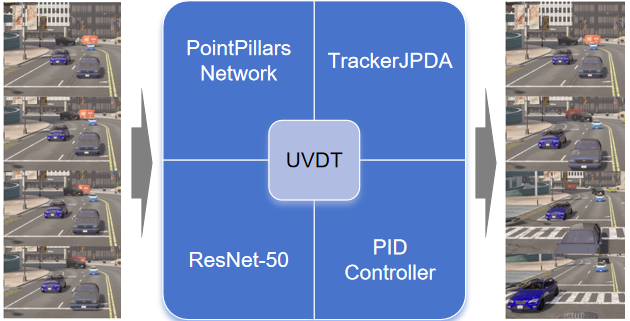
\includegraphics[width=\columnwidth]{picture/picture1.eps}}
	\caption{The overall preview of the digital twin is provided through UVDT. The technical process from real vehicle trajectory to digital twin trajectory and traffic flow simulation is demonstrated.}
	\label{fig1}
\end{figure}

However, the digital twin system faces several key technical bottlenecks in the process of achieving high-fidelity traffic scene modeling.
First, the problem of multi-target tracking in complex urban scenes is particularly prominent. Frequent target detection failures caused by factors such as mutual occlusion between vehicles, extreme changes in lighting conditions, and sudden changes in sensor viewing angles seriously affect the system's continuous and accurate estimation of the dynamic state parameters of traffic participants\cite{Alpher23c}.
Second, the performance of multi-source heterogeneous sensors is significantly restricted by environmental conditions. Specifically, under severe meteorological conditions, the electromagnetic wave attenuation of millimeter-wave radars shortens the effective detection distance; while in low-light environments, vision-based perception systems face the technical difficulty of a sharp drop in image signal-to-noise ratio.
In particular, the identity switching problem in the multi-target tracking process will destroy the spatiotemporal continuity of traffic flow, which will lead to deviations in the system's behavior prediction and decision-making in complex scenes such as intersections.
In addition, the time series asynchrony problem caused by non-real-time data processing will cause cumulative errors in the prediction model, ultimately resulting in a progressive mismatch between the digital twin system and the physical world.
These technical challenges have largely limited the engineering application value of digital twin technology in autonomous driving system verification and intelligent traffic management.

In response to the above problems, this study conducts research from four dimensions: multi-object tracking at a single intersection, multi-object tracking at multiple intersections, trajectory inference and restoration, and digital twin system construction, as shown in Fig. \ref{fig1}. 
First, the object-level fusion detection method based on cameras and LiDAR is used to improve vehicle detection accuracy and thus enhance tracking robustness. 
At the same time, the Re-identification (ReID) technology is introduced to achieve identity association across camera scenarios through vehicle appearance features (such as skeleton models, color changes, etc.), effectively solving the ID switching problem and ensuring trajectory continuity and consistency under complex lighting and occlusion conditions\cite{Alpher23}. 
Secondly, in terms of trajectory reasoning, relying on the efficient navigation algorithm framework of the CARLA simulation platform, the shortest path planning strategy is used for trajectory inference. 
This method has the advantages of high computational efficiency, strong environmental adaptability, and controllable errors. 
Finally, the integrated control algorithm is used to accurately simulate vehicle driving behavior, and a complete autonomous driving system verification platform is constructed to provide a high-fidelity digital twin foundation for algorithm development and safety assessment\cite{Alpher24c}.

\section{Related Work}

We have summarized research work on different aspects of UVDT.

\textbf{Multi-Object Tracking.}
The development of multi-object tracking technology depends largely on the performance improvement of front-end object detection.
In recent years, detection methods based on multi-sensor fusion have provided more reliable data input for tracking systems.
MVDNet (2018) effectively improves the detection accuracy in complex environments by fusing LiDAR point clouds and camera images through multi-view projection\cite{Alpher22h}.
Building on this, PointPillars introduces a fast encoder for LiDAR data, using a grid-based encoding approach that could potentially be integrated with camera data in future fusion methods to enhance detection speed and efficiency\cite{Alpher19}.
We use a combination of PointPillars-based 3D point cloud detection method and YOLOv4-based 2D image detection method for multimodal object detection.

In terms of tracking algorithms, researchers have proposed a variety of innovative methods.
Specker and his team proposed an online multi-camera multi-object tracking method, which dynamically optimizes cross-camera target association through an innovative Corrective Matching Cascade strategy, significantly improving tracking accuracy and ID consistency in complex scenarios while ensuring real-time processing\cite{Alpher24e}.
Shim and his team proposes a robust multi-target multi-camera vehicle tracking system designed for city-scale traffic management, addressing challenges like occlusion and cross-camera identity consistency by integrating spatial-temporal constraints and deep feature fusion to enable real-time vehicle monitoring and behavior analysis across urban camera networks\cite{Alpher21e}.
Most existing algorithms, with a few exceptions, can be seen as special cases of the multi-modal fusion problem. 
These methods organize the input data using a graph structure, where edges represent relationships between modalities, and nodes represent different targets or states. 
Algorithms that can be solved in polynomial time typically handle specific modalities or time-continuous edges, with some also utilizing maximum flow or matching algorithms. 
Methods that leverage global information (beyond just time continuity or modality constraints) can significantly improve performance, but they are usually NP-hard due to the involvement of combinatorial optimization. 
In some cases, marginal terms or local constraints are added to ensure completeness. 
To enhance model expressiveness, some studies have employed higher-order relations, although the gains diminish significantly as complexity increases. 
Joint optimization and iterative optimization strategies have also been widely used to improve performance.
We use Joint Integrated Probabilistic Data Association (JIPDA), which combines data from multiple sensors and optimizes probabilistic associations to effectively handle data uncertainty and missing information in target tracking, improving tracking accuracy and robustness in complex environments.

\begin{figure*}[t]
	\centerline{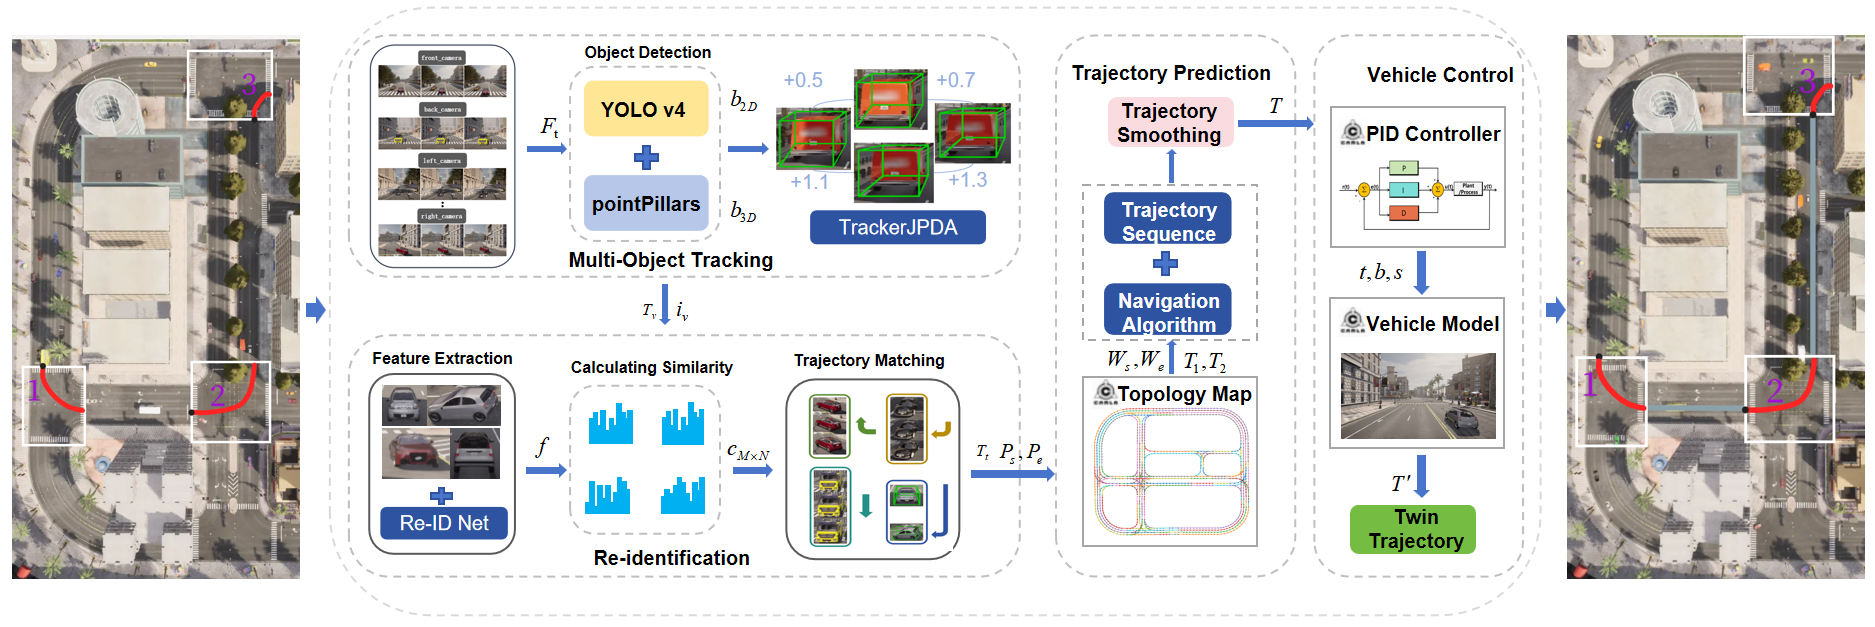
\includegraphics[width=\textwidth]{picture/picture2.eps}}
	\caption{In the given scenario, synchronized cameras and LiDAR sensors detect vehicles, while the tracking system performs both single-intersection and multi-intersection multi-object tracking. The tracking data is subsequently utilized for trajectory reconstruction, ultimately enabling the creation of a digital twin that accurately replicates the traffic scenario. Where \(W_{s}\) and \(W_{e}\) are the coordinates of the endpoints of the tracked trajectory in the simulation scenario, and \(T_{1}\) and \(T_{2}\) are the trajectories tracked at different intersections.}
	\label{fig2}
\end{figure*}

\textbf{Vehicle ReID.}
Bing and his team proposed a part-based regularization method, which enhances the accuracy of vehicle re-identification by detecting local parts of vehicles, such as lights and wheels\cite{Alpher19b}. 
Zheng and his colleagues introduced a large-scale vehicle re-identification dataset named VehicleNet and proposed a multi-task learning framework that combines vehicle re-identification and vehicle attribute recognition tasks, improving the model's generalization capability\cite{Alpher20f}. 
Khorramshahi and the research team proposed a dual-path model that integrates global and local features and incorporates an adaptive attention mechanism to enhance the accuracy of vehicle re-identification\cite{Alpher19c}.

The most advanced technologies in the field of vehicle re-identification currently include the combination of deep Convolutional Neural Networks (CNN) for feature extraction and metric learning\cite{Alpher20g}, particularly with the integration of cross-view and cross-domain learning techniques, the use of Generative Adversarial Networks (GAN) for image enhancement\cite{Alpher21d}, and the fusion of multi-sensor data (such as cameras, radar, and LiDAR) to improve the model's robustness and accuracy in complex environments\cite{Alpher22g}.

Inspired by person ReID techniques for video sequences, we developed a retrained vehicle ReID network based on ResNet-50. 
The network has acquired comprehensive feature representations through large-scale image training, enabling effective vehicle re-identification performance.

\textbf{Digital Twin.}
After obtaining the trajectory data of all tracked vehicles, we will use the vehicle control algorithm to reproduce the traffic flow in the simulation scenario.
Kaleb Ben Naveed et al. proposed a hierarchical reinforcement learning-based method for autonomous driving trajectory planning and control. 
By training a reinforcement learning agent in a simulation environment, this method optimizes the vehicle's control strategy according to environmental changes, achieving efficient trajectory planning and dynamic path adjustment.\cite{Alpher22}
R. Barea et al. proposed a Deep Reinforcement Learning (DRL)-based control method, where an agent is trained in the CARLA simulation platform to autonomously learn and optimize the vehicle's control strategies (such as throttle, brake, and steering) to ensure safe and smooth driving.\cite{Alpher21}
We optimize the trajectories obtained from multi-object tracking using a trajectory smoothing algorithm, enabling the vehicle to turn more smoothly and drive more steadily (reducing bumps and sudden maneuvers) while ensuring precise adherence to the planned path at a lower computational cost. 
Subsequently, the PID controller is employed to control the vehicle, guiding it to follow the optimized trajectory and achieve final trajectory-tracking synchronization.


\section{Method}

\subsection{Problem Definition}

In UVDT, the vehicle detection and tracking system for single-intersection scenarios adopts a multimodal data fusion architecture.
As illustrated in Fig. \ref{fig2}, the input source \(F_{t}\) integrates 3D point cloud data captured by LiDAR and synchronized RGB images from six calibrated cameras, achieving heterogeneous sensor data collaboration through spatiotemporal alignment.
The tracker generates the vehicle trajectory \(T_{v}\) of a single intersection and the image \(i_{v}\) of the corresponding vehicle through the detection bounding boxes \(b_{2D}\) and \(b_{3D}\) obtained by object detection algorithms.
For cross-intersection vehicle trajectories matching, we employ a re-identification network to extract appearance feature vectors \(f\), then compute their cosine similarity to produce a logical matching matrix \(C_{M \times N}\).
Vehicle trajectories exceeding a predefined similarity threshold are matched and output as \(T_{t}\).
The system subsequently feeds trajectory endpoints \((P_{s},P_{e})\) to a prediction framework that interpolates inter-intersection trajectories, ultimately producing complete vehicle trajectories \(T\). 
The controller calculates throttle\(t\), brake\(b\),and steering wheel \(s\) outputs from these trajectories to guide vehicle control, with the final executed trajectory denoted as \(T^\prime\).

\textbf{Vehicle Detection in Point Clouds.}
Based on the PointPillars network architecture, 3D vehicle detection in intersection scenarios is implemented. Its input data is collected in real time through a 64-line laser radar (range measurement: 200m, point cloud density: 2.2M pts/s, scanning frequency: 20Hz), and the 3D ground truth information of vehicles in the range is recorded simultaneously. The original dataset is divided into a training set and a test set in a 7:3 ratio. The training set is used to learn the mapping relationship from point cloud to 3D detection box, and the test set verifies the generalization ability of the model on unknown data.

A PointPillars network requires two inputs: pillar indices as a P-by-2 and pillar features as a P-by-N-by-K matrix. P is the number of pillars in the network, N is the number of points per pillar, and K is the feature dimension.
The network begins with a feature encoder, which is a simplified PointNet. It contains a series of convolution, batch-norm, and relu layers followed by a max pooling layer. A scatter layer at the end maps the extracted features into a 2-D space using the pillar indices.
Next, the network has a 2-D CNN backbone that consists of encoder-decoder blocks. Each encoder block consists of convolution, batch-norm, and relu layers to extract features at different spatial resolutions. Each decoder block consists of transpose convolution, batch-norm, and relu layers.
The network then concatenates output features at the end of each decoder block, and passes these features through six detection heads with convolutional and sigmoid layers to predict occupancy, location, size, angle, heading, and class.

\textbf{Trajectory Association between Intersections.}
Multi-intersection trajectory association is essentially a multi-dimensional combinatorial optimization problem, and its complexity grows exponentially with the increase in the number of monitoring nodes and targets.
Due to the differences in observation angles, occlusion conditions, and sensor performance at different intersections, targets often have inconsistent feature representation when they move across intersections.
Especially in complex scenarios, when targets are temporarily occluded or leave the sensor's field of view, traditional tracking algorithms often have difficulty maintaining the continuity of target identity.
These limitations seriously affect the fidelity and reliability of digital twin models.

To solve this problem, we adopt a strategy that combines deep feature matching with global optimization, extracts multimodal feature representations with strong discriminability through the CNN architecture, and constructs a spatiotemporal constraint graph for global association optimization.
In terms of specific implementation, the system first obtains a unified feature representation of the target through deep metric learning, which can effectively overcome the domain differences between different cameras.
Then, a hierarchical optimization framework is used to generate candidate association pairs based on feature similarity at the bottom layer, and global consistency verification is performed at the upper layer in combination with kinematic constraints and road network topology.

This method can not only effectively alleviate the tracking interruption problem caused by the short disappearance of the target, but also improve the target consistency maintenance ability of the digital twin system in long time sequence scenarios, providing a more robust perception basis for applications such as autonomous driving and intelligent monitoring.\cite{Alpher24d}.

\subsection{Single Intersection Multi-Object Tracking}

We fuse detections from our LiDAR and cameras at a single intersection and use the tracker JDPA object to track the target.

\textbf{Single Detection Class Probability Update.}
The tracker adopts a recursive state estimation framework to propagate and update the target states from the previous time step \(k-1\) to the current time step \(k\).
\(\mu_i(k-1)\) represents the state vector estimate of the \(i\)-th target at time \(k-1\), while \(\mu_i(k)\) represents the combined state estimate of all targets at time \(k\).
The operation \(\otimes\) represents the element-wise multiplication between state vectors, while \(c_{j}\) serves as a normalization factor for category \(j\) to dynamically adjust the relative weights of different objectives during the fusion process.
This mathematical representation captures the essential mechanism for maintaining consistent multi-object tracking through temporal state propagation and weighted information fusion.
The normalization procedure ensures numerical stability while preserving the probabilistic interpretation of the state estimates, which is particularly crucial when dealing with target interactions and measurement uncertainties in complex tracking scenarios.

\begin{align}
	\mu(k) & = \frac{c_{j} \otimes [ \mu_1(k-1), \ldots, \mu_N(k-1) ]^T}{c_{j}^{T} [ \mu_1(k-1), \ldots, \mu_N(k-1) ]^T}
\end{align}

\textbf{Mixed Association Likelihood in Cluster.}
A state update method based on kernel function fusion is used to solve the problem of mutual occlusion and trajectory intersection between targets leading to reduced tracking performance.
\(\Lambda_{k}\) mainly captures the motion characteristics of the target, \(\Lambda_{c}\) extracts the appearance characteristics of the target, and \(\Lambda(m, t)\) represents the comprehensive evaluation value of the target state in detection \(m\) and trajectory \(t\).
\begin{align}
	\Lambda(m, t) & = \Lambda_{k}^{1-\alpha}(m, t) \Lambda_{c}^{\alpha}(m, t)
\end{align}
The parameter \(\alpha\) plays a key regulatory role here. By dynamically adjusting the value of \(\alpha\), the relative contribution weights of motion features and appearance features in the tracking process can be flexibly balanced.
\begin{align}
	\Lambda_{c}(m, t) = \left\{\begin{array}{ll}
		c_{j}^{T}\left[\mathbb{I}_t \mu(k-1)+\mathbb{I}_{t = 0} \mu^{0}\right] & \text { if } m>0 \\
		1 & \text { if } m = 0
	\end{array}\right.
\end{align}
The hybrid association likelihood function achieves multi-scenario adaptive matching through a triple mechanism: for valid associated targets (\(m>0\) and \(t>0\)), the system corrects the trajectory category probability distribution \(\mu(k-1)\) in real time through Bayesian updating, and uses the confusion matrix column vector \(c_j\) of the detection m corresponding to category \(j\) to calculate the matching degree, thereby dynamically adapting to changes in target categories; for new targets (\(m>0\) and \(t=0\)), the prior distribution \(\mu^{0}\) based on the statistical characteristics of the data set is used for initialization to effectively solve the cold start problem; for unmatched trajectories (\(m=0\)), a fixed value of 1 is returned to avoid false termination caused by sensor noise. The design achieves the optimal fusion of kinematics and category information through the \(\alpha\) parameter, significantly improving the tracking robustness in complex scenarios while ensuring real-time performance.

\textbf{Update Track Class Probability.}
When processing a set of detection results, each tracking target maintains a set of marginal probabilities \(\left(P_{0}, P_{1}, \ldots, P_{M}\right)\), which represent the association likelihood between the target and the \(M\) available detection results in the current frame. Here, \(P_{0}\) specifically denotes the probability that the target is not associated with any detection result in the current frame.
\begin{align}
	\mu_{k} & = \left(\sum_{m = 1}^{M} P_{m} \frac{c_{j(m)} \otimes \mu(k-1)}{c_{j(m)}^{T} \mu(k-1)}\right)+ P_{0} \mu(k-1)
\end{align}
The tracker sequentially updates the trajectory classification attributes on a cluster-by-cluster basis. 
Where \(c_{j}(m)\) is the class probability vector of detection \(m\) corresponding to category \(j\), \(\otimes\) represents element-wise multiplication, \(\mu(k-1)\) is the class probability vector for the \((k-1)\)-th step, and \(\mu(k)\) is the class probability vector for the \(k\)-th step.

\textbf{Process.}

In this process, we employ a tracker to handle the 2D and 3D bounding boxes obtained from target detection, along with their corresponding timestamps. 
The tracker utilizes a soft assignment strategy, allowing each trajectory to integrate contributions from multiple detection results. 
Its responsibilities include trajectory initialization, confirmation, correction, prediction (including prediction in a coasting state without active motion), and deletion. 
For each trajectory, the tracker estimates its state vector and the covariance matrix of the state estimation error. 
It ensures that every detection is assigned to at least one trajectory; if a detection cannot be matched to any existing trajectory, the tracker creates a new one.

Newly generated trajectories are initially in a tentative state. 
When a tentative trajectory accumulates a sufficient number of detection assignments, its status transitions to confirmed. 
If the detections themselves already carry explicit classification information (i.e., the returned trajectory data contains non-zero fields), the corresponding trajectory is immediately confirmed as valid. 
Once a trajectory is confirmed, the tracker recognizes it as representing a real physical object. 
However, if a trajectory fails to receive any detection assignments within a predefined number of update cycles, it will be deleted.

Through this process, we are ultimately able to obtain the trajectories of vehicles within the intersection.

\textbf{Reference System.}

We placed an imaginary ego-vehicle in the center of the intersection, which serves as a reference system, as shown in Fig. \ref{fig3}. 
For multi-object tracking we input not only the detection frame, but also the position of the camera and radar relative to the self-vehicle, as well as the position of the ego-vehicle. 
The position coordinates of the self-vehicle in the experiment were always O(0,0,0), i.e. stationary. 
Tracking initially generates trajectory coordinates \(\text P_1\) relative to the LiDAR, which we also fit to the world coordinates \(\text P_2\) in the simulation scenario.
\begin{figure}[!t]
	\centerline{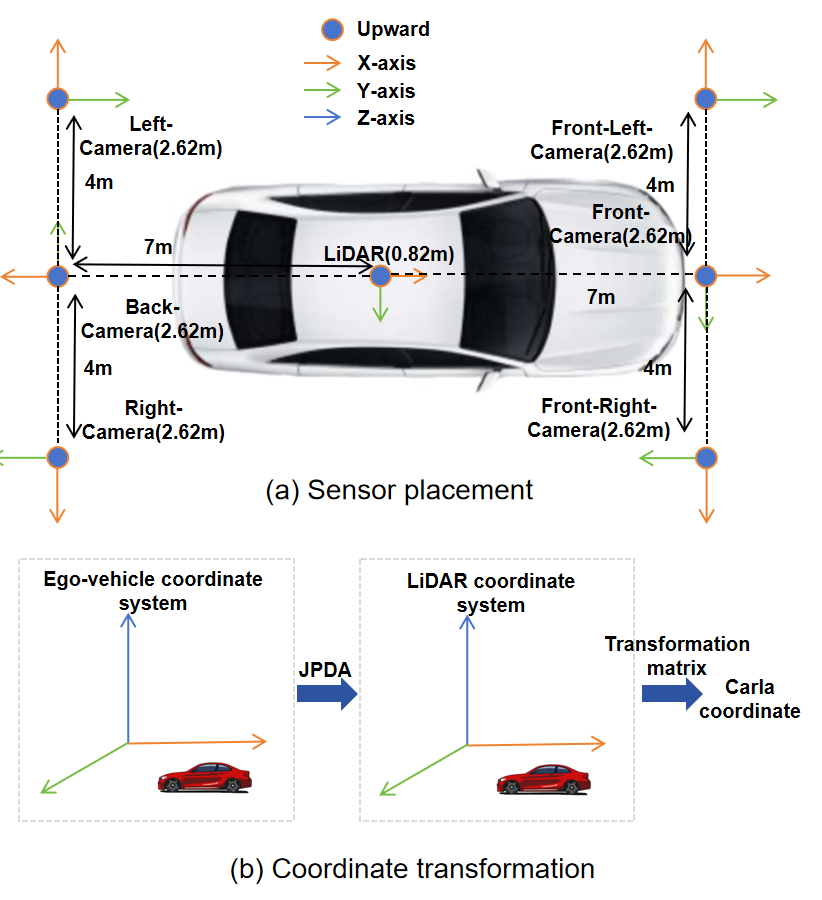
\includegraphics[width=\columnwidth]{picture/picture3.eps}}
	\caption{Sensor configuration and coordinate transformation process: (a) Multi-sensor arrangement on the ego vehicle, including 6 cameras (2.62 meters upward offset) and 1 lidar (0.82 meters upward offset); (b) Coordinate transformation process from the ego vehicle system (left) to the lidar coordinate system (right) through JPDA, and finally converted to world coordinate in the simulation scenario through the transformation matrix. All distance measurements are in meters.} 
	\label{fig3} 
\end{figure}

\subsection{Multi Intersection and Multi-Object Tracking}

In the simulation scenario, we configure a differentiated blueprint for each experimental vehicle, so that it strictly follows the preset path from a fixed starting point to a specified end point, and build a fully controllable and highly reproducible dynamic traffic scenario.
To achieve all-round data collection, we deploy RGB cameras and semantic segmentation cameras at the front and rear positions of each experimental vehicle, respectively, and use a multi-view synchronous acquisition system to capture the continuous changes in the vehicle's appearance features and spatial posture in real time, and finally generated dynamic ground truth and image sequences with precise spatiotemporal alignment characteristics.

Subsequently, the vehicle images of the front and rear views are cropped based on ground truth and the front and rear view images of the same vehicle are combined to form a dataset of that vehicle, to which the vehicle images of the occluded views are added to form the final dataset.
Before training the re-identification network, the images were reshaped to a size of 224\(\times\)224, of which 90\% were used as training sets and the rest as validation sets.

Finally, the vehicle images tracked between intersections are matched through the trained re-identification network.
In other words, the vehicle tracked at the previous intersection is the object that needs to be re-identified, and it will be recognized at the next intersection, allowing the trajectories corresponding to the two vehicles to be integrated.

For matching vehicle trajectories between intersections, we use a re-recognition network to extract features from the vehicle images and then compute the cosine similarity of these two features.
If Intersection 1 has M vehicles and Intersection 2 has N vehicles, a matrix of size M×N is generated. 
If the similarity exceeds a certain threshold, the two vehicles are considered to be the same vehicle.

\textbf{ResNet-50.}
ResNet-50 mainly consists of five main parts: initial convolutional layer, maximum pooling layer, four-stage residual block, global average pooling layer and fully connected layer, totaling 50 layers, of which the four-stage residual block is its core. The first residual block of each stage downsamples the size of the feature map, while the subsequent residual blocks keep the size of the feature map unchanged. We use the pre-trained version and as the backbone network of the re-identification network, it has learned rich feature representations based on a large number of images.

\subsection{Trajectory Inference and Reconstruction}

\textbf{Inference of Trajectories in Unknown Regions.}
Upon completing the tracking of all vehicle trajectories, we chronologically sort the trajectory of each vehicle and select the last waypoint of the same vehicle at the previous intersection along with the first waypoint at the next intersection as the starting and ending points of the unknown region. 
These two waypoints are then fed into the navigation algorithm module, which subsequently computes the trajectory between them.

In the simulation environment, vehicle trajectory planning is achieved by utilizing the A* algorithm to search for the shortest path within the graph structure constructed from the topological map. 
The A* algorithm evaluates the comprehensive cost of nodes and, at each step, selects the node with the lowest comprehensive cost for expansion, thereby effectively guiding the current node \(p_{n}\) to search for the target node \(p_{g}\).
The core of this algorithm lies in the following evaluation function. 
\begin{align}
	f(n) = \sum_{k = 1}^{n} \frac{d_{k} \cdot\left(1+\alpha \phi_{k}\right)}{1 + \frac{\gamma}{\kappa_k + \epsilon}}+\left\|\left[\begin{array}{c}
		p_{n}-p_{g} \\
		\sqrt{\lambda}\left(l_{n}-l_{g}\right)
	\end{array}\right]\right\|_{2}
\end{align}
Its purpose is to calculate the actual cost from the starting node to the current node and the estimated cost from the current node to the target node. 
In the process of exploring the shortest path using the A* algorithm, if there are edges with a weight of 0 in the graph structure, it may cause the vehicle to change lanes too frequently in a very short time, which contradicts the normal driving logic. 
To alleviate this phenomenon, we introduced a lane change penalty mechanism in path planning. Specifically, when the current lane \(l_{n}\) is inconsistent with the target lane \(l_{g}\), the calculation cost will be increased to ensure that the distance calculation between nodes is not only based on the spatial distance, but also takes into account the frequency of lane changes. Not only that, when calculating the inter-node distance \(d_{k}\), we also added a road type penalty \(\phi_{k}\) and a curvature penalty \(\kappa_k\). When planning the route globally, the vehicle prefers the main road and the road with smaller curves. 
Among them, \(\alpha\) represents the road attribute weight, \(\gamma\) controls the curvature penalty intensity, \(\lambda\) is the lane matching weight, and \(\epsilon\) is used as a regularization parameter to ensure numerical stability.


\textbf{All Trajectory Restoration.}
Through the aforementioned algorithmic framework, we are able to obtain vehicle trajectories in unknown regions. 
Simultaneously, we have also acquired vehicle trajectories at intersections using the JPDA tracker. 
At this point, we only need to concatenate all trajectories of the same vehicle in chronological order and place them into a new collection, thereby obtaining the complete trajectory of that vehicle. 
This method can be represented as: 
\begin{align}
	S(t) = \bigcup_{i=1}^{N} \Bigl( T_i(t) \cup f\Bigl( \lim_{\!t \to t_i^+} T_i(t), \lim_{\!t \to t_{i+1}^-} T_{i+1}(t) \Bigr) \Bigr)
\end{align}
where \(S\) is the trajectory collection, \(T_i(t)\) represents the \(i\)-th trajectory. 
The limits \(\lim_{t \to t_i^+} T_i(t)\) and \(\lim_{t \to t_{i+1}^+} T_{i+1}(t)\) correspond to the end waypoint of the \(i\)-th trajectory and the start waypoint of the \((i+1)\)-th trajectory, respectively.
As demonstrated in Fig. \ref{fig5}, we can derive the complete vehicle trajectory collection, effectively reconstructing the trajectories of all vehicles.
\begin{figure}[!t]
	\centerline{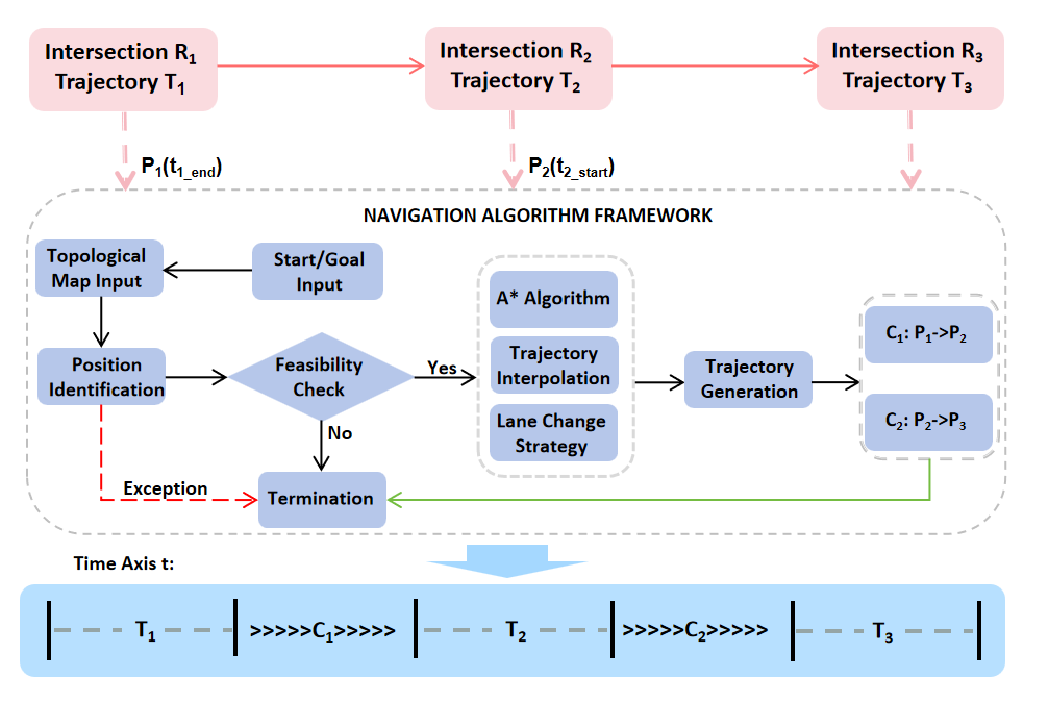
\includegraphics[width=\columnwidth]{picture/picture5.eps}}
	\caption{Trajectory restoration diagram, showing how to generate predicted trajectories between intersections from multi-object tracking trajectories and then obtain the complete vehicle trajectory.} 
	\label{fig5} 
\end{figure}

\subsection{Twin of Trajectory}

Through the previous steps, we have obtained the trajectories of all vehicles. 
Here, we will further optimize these trajectories using a trajectory smoothing algorithm, and then employ a PID controller to control the vehicles, ensuring they follow the optimized trajectories\cite{Alpher22d}. 

A trajectory smoothing method based on linear interpolation is adopted in this work.
Given the original trajectory point set \(W = \{w_1,w_2 ,…,w_n\}\), where \(w_i \in R^2\) represents the coordinates of the \(i\)-th track point, the smoothed track \(\widetilde{W}\) is generated by:
\begin{align}
	\widetilde{W} = \bigcup_{i = 1}^{n-1} \left( w_i \cup \left\{ w_i + k\delta \cdot \frac{w_{i+1} - w_i}{d_i} \ \middle|\ k \in \mathbb{N}^+\right\} \right)
\end{align}
Precise control of trajectory density is achieved through a step size parameter \(\delta\) in this method, which maintains strict adherence to the original trajectory geometry and ensures all interpolation points are positioned on line segments connecting adjacent original waypoints.
Specifically, for any adjacent waypoint pair, the algorithm uniformly inserts new waypoints on its connection line. The number of insertion points is dynamically determined by the ratio of distance \(d_i\) to step \(\delta\), and the constraint \(k\delta < d_i\) is satisfied, thereby ensuring the adaptive matching of the interpolation density and the local geometric features of the trajectory.
It is worth noting that the current method assumes that the input waypoints are all on the real trajectory, and for the filtering of possible external or noise points, an additional robust processing mechanism is needed, which will be an important direction for future research.

The PID controller consists of three main components: Proportional control (P), Integral control (I), and Derivative control (D). Each component serves a specific purpose, enabling the regulation of different aspects of the system.

\begin{align}
	u = K_p e + K_i \int \left( e - \frac{\text{sat}(u)-u}{K_p} \right) dt + K_d \dot{e}
\end{align}
This study proposes an improved PID control algorithm, whose control output \(u\) consists of proportional term, anti-saturation integral term, and differential term, where \(K_p\), \(K_i\) and \(K_d\) are proportional gain, integral gain and differential gain respectively.
The algorithm achieves rapid error response through the proportional term, eliminates steady-state errors using the integral term, and suppresses the error change rate through the differential term.
Experimental studies have shown that traditional PID control has an integral saturation phenomenon in the vehicle steering system, resulting in random extreme deflections of the steering wheel (±1 rad).
To this end, this algorithm introduces a compensation term, and the saturation function sat(u) limits the controller output \(u\) to a preset interval [\(u_{min}\), \(u_{max}\)].
When the control output reaches the saturation limit, the integral accumulation rate is automatically adjusted, which effectively solves the integral saturation problem.
Here, \(\dot{e}\) represents the rate of change of the error over time.

The tuning process of the PID controller is as follows:  
1. Calculate the error \(e\) between the target value (setpoint) and the current system output in real time.  
2. Compute the proportional action based on the current error, the integral action based on historical errors, and the derivative action based on the rate of change of the error.  
3. Sum the results of the proportional, integral, and derivative components to obtain the final control output, which is then applied to the system (for example, adjusting the vehicle's acceleration or direction). 
4. The system adjusts based on the control output, changing its state (for example, speed, position, etc.). 
The controller continues to monitor the system state, updates the error in real time, and repeats the above steps until the system stabilizes near the target value.


\subsection{Evaluation}

We employed three evaluation metrics.

\textbf{Multiple Object Tracking Accuracy.}
Single-camera, multi-object tracking performance is typically measured by the Multiple Object Tracking Accuracy \((MOTA)\)\cite{Alpher23b}.
We use an improved evaluation metric Robust Multi-Object Tracking Accuracy \((RMOTA)\) based on sliding window median statistics, which aims to enhance the robustness of traditional \(MOTA\) to short-term occlusion and ID switching.
The tracking sequence is divided into \(W\) time windows, and each window independently calculates the local \(MOTA\) score to avoid the serious error of a single frame affecting the overall evaluation.
In addition, the penalty for identity mismatching is amplified by the coefficient \(\alpha\) to reflect the key impact of ID continuity on tracking quality.
\begin{align}
	RMOTA = \underset{i=1}{\overset{W}{\mathrm{median}}} \left(1 - \frac{FN^{(i)} + FP^{(i)} + \alpha M^{(i)}}{T^{(i)}}\right) 
\end{align}
Among them,
\(FN^{(i)}\) (False Negatives) represents the number of missed detections in the \(i\)-th window, which means targets that truly exist but were not detected.
\(FP^{(i)}\) (False Positives) represents the number of false detections in the \(i\)-th window, which means targets that were detected but do not actually exist.
\(M^{(i)}\) (Mismatches) represents the number of identity mismatches in the \(i\)-th window, which means cases where the tracking ID of a target was incorrectly assigned during the tracking process.
\(T^{(i)}\) (Total Number of True Detections) represents the total number of true detections in the \(i\)-th window, which means the number of targets correctly detected across all frames.

The metric ranges from 0 to 1, with higher values indicating better tracking performance. 
A perfect score of 1 represents flawless tracking with zero missed detections, false alarms, or identity mismatches, while 0 indicates complete tracking failure.

\textbf{Cross-Sensor Tracking Accuracy.}
Multi-Camera Object Tracking Accuracy \((MCTA)\)\cite{Alpher23b} condenses all aspects of system performance into a metric that measures cross-camera tracking.
On this basis, this paper proposes an Interpretable Multi-Camera Object Tracking Accuracy \((IMCTA)\), which is defined as follows:
\begin{align}
	IMCTA = {\frac{2PR}{P + R}}_{\text{}} \times \prod_{k \in \{w, h\}} \left(1 - \frac{M_k + \lambda E_k^{\text{ID}}}{T_k}\right)
\end{align}
by decomposing the cross-camera error into missing association \(M_k\) and ID switching \(E_k^{\text{ID}}\), accurate diagnosis of system defects is achieved.
Among them,
\(P\) represents the proportion of correct matches (correctly identifying and tracking targets) across all cameras.  
\(R\) represents the recall rate, which is the proportion of all true targets that are correctly tracked.  
\(\lambda\) is the penalty coefficient for ID switching error and \(T^{k}\) represents the total number of potential correct associations in the \(k\)-th dimension, and \(w\) and \(h\) represent within-intersection and between-intersection, respectively.

Compared with \(MCTA\), \(IMCTA\) intuitively demonstrates the independent evaluation and synergy of detection capability and cross-camera association capability, transforming complex cross-camera evaluation into a transparent framework that is quantifiable, adjustable, and diagnosable. 
The higher the value, the better the performance of the multi-camera tracking system.

\begin{table*}[t]
	\centering
	\caption{MULTI-OBJECTIVE TRACKING EVALUATION}
	\label{tab:2}
	\small
	\begin{tabular}{@{}l@{\hspace{1em}}c@{\hspace{0.5em}}*{10}{r}@{}}
		\toprule
		\textbf{Scene} & \textbf{Int.} & \textbf{Rcll} & \textbf{Prcn} & \textbf{FTR} & \textbf{FP} & \textbf{FN} & \textbf{IDS} & \textbf{MT} & \textbf{ML} & \textbf{RMOTA} & \textbf{RMOTP} \\
		\midrule
		\multirow{5}{*}{\shortstack[l]{Town01 \\ (16 intersections, f- \\ lat roads, sparsely \\ populated buildings)}} 
		& 1 & 30.1025 & 59.9258 & 0.5106 & 216 & 750 & 18 & 0.0000 & 37.5000 & 8.2945 & 79.9222\\
		& 2 & 64.8065 & 61.5385 & 1.0297 & 450 & 391 & 21 & 55.5556 & 33.3333 & 22.4122 & 86.7746\\
		& 3 & 63.2135 & 45.4407 & 1.1887 & 359 & 174 & 15 & 0.0000 & 25.0000 & -15.8562 & 86.9053\\
		& 4 & 65.8206 & 96.7662 & 0.0369 & 13 & 202 & 20 & 40.0000 & 20.0000 & 60.2369 & 89.0919\\
		& 5 & 41.4035 & 90.0763 & 0.0580 & 13 & 167 & 10 & 50.0000 & 0.0000 & 33.3333 & 88.2471\\
		\midrule
		\multirow{5}{*}{\shortstack[l]{Town10 \\ (7 intersections, hig- \\ h-density, including \\ steep slopes)}} 
		& 1 & 30.6653 & 59.7166 & 0.7960 & 398 & 1334 & 28 & 8.3333 & 50.0000 & 8.5239 & 84.6488\\
		& 2 & 56.4410 & 70.6095 & 1.1380 & 569 & 1055 & 29 & 13.3333 & 26.6667 & 31.7506 & 81.0920\\
		& 3 & 51.9805 & 75.6714 & 0.6160 & 308 & 885 & 17 & 14.2857 & 35.7143 & 34.3462 & 84.2826\\
		& 4 & 52.1930 & 86.1427 & 0.2680 & 134 & 763 & 50 & 27.2727 & 36.3636 & 40.6642 & 88.6035\\
		& 5 & 45.4243 & 62.2719 & 1.6540 & 827 & 1640 & 35 & 12.5000 & 37.5000 & 16.7388 & 86.0825\\
		\bottomrule
	\end{tabular}
\end{table*}

\textbf{Twin Accuracy.}
In the twin experimental evaluation, we verify the effectiveness of the system by comparing the comprehensive performance of the following three key trajectories: (1) the actual trajectory of the vehicle, (2) the observed trajectory reconstructed based on the multi-object tracking algorithm, and (3) the expected trajectory generated by the control system.
This study uses Trajectory Overlap Ratio (TOR) for comprehensive evaluation, which quantifies both the shape similarity of the trajectory and the spatiotemporal consistency of the waypoints.
\begin{align}
	TOR & = \left(1 - \frac{D_{dtw}}{D_{max}}\right) \times \Lambda(t)
\end{align}
Among them, the shape similarity term is calculated based on the ratio of the dynamic time warping distance \(D_{dtw}\) to the maximum scale distance \(D_{max}\), reflecting the overall geometric difference of the trajectory, while the spatial alignment term \(\Lambda(\tau)\) evaluates the static matching accuracy of the waypoint through the position offset penalty.
This evaluation mechanism can not only capture the morphological differences of macroscopic paths, but also characterize the spatiotemporal consistency of discrete waypoints at the micro level, providing a multi-dimensional quantitative basis for the trajectory consistency of the digital twin system.
\begin{align}
	D_{dtw} = \min_{\pi \in P} \sqrt{\sum_{(i,j)\in\pi} \|p_i - q_j\|^2}
\end{align}
\begin{align}
	D_{max} = \max_{i,j} \|p_i - q_j\| \cdot \max(n,m)
\end{align}
\(D_{dtw}\) compares the similarity of non-aligned sequences through a dynamic curved path \(\pi\), and finds the matching solution that minimizes the cumulative distance from all possible path sets \(P\), while \(D_{max}\) quantifies the spatial deviation of the two trajectories in the worst case and normalizes it by the trajectory length. Among them, \(p_{i}\) and \(p_{j}\) represent the matching point pairs of the two trajectories, and \(m\) and \(n\) are the lengths of the two trajectories respectively.

\begin{align}
	\Lambda(\tau) = \frac{1}{n} \sum_{k=1}^{n} \mathbb{I}\left(\left\|p_{\pi_{1}(k)}-q_{\pi_{2}(k)}\right\| \leq \tau\right)
\end{align}
The trajectory we finally get is the coordinates in the simulation scenario, which means that the trajectory is actually discrete.
Therefore, calculating the positional relationship between waypoints is very important to reflect the overlap between two trajectories.
\(\Lambda(\tau)\) counts the proportion of matching points in the two trajectories whose distance is less than the threshold \(\tau\) to reflect the overlap accuracy of the two trajectories within the allowable error range.
where \(p_{\pi_{1}(k)}\) and \(q_{\pi_{2}(k)}\) represent the three-dimensional coordinates of the \(\pi_{1}(k)\)th point of trajectory 1 and the \(\pi_{2}(k)\)th point of trajectory 2, respectively, and \(\mathbb{I}(\cdot)\) is the indicator function (which takes the value of 1 when the Euclidean distance between two points does not exceed the threshold \(\tau\), otherwise it takes the value of 0).


\section{Experiments}

\subsection{Preparation}

\textbf{Simulation Environment.}
We conducted simulation experiments in CARLA, whose advantage lies in its provision of a highly realistic virtual environment capable of accurately simulating complex traffic scenarios and diverse driving conditions. 
CARLA supports flexible sensor configurations, such as cameras and LiDAR, facilitating multimodal data acquisition and fusion experiments\cite{Alpher22e}. 
We conducted relevant experiments in the Town10 and Town01 scenarios in CARLA.
The complex urban structure and dense traffic flow of Town10 can simulate highly dynamic real traffic environments, while the simple layout and clear rules of Town01 make it easy to construct controlled experimental scenarios.
This scenario diversity can effectively verify the generalization ability of the model under different traffic conditions and provide a reliable basis for actual road deployment.

\textbf{Data Collection.}
In CARLA's Town10 scenario, a single intersection location is selected, with a LiDAR placed at the center and six cameras arranged around it to achieve 360-degree omnidirectional perception coverage. 
This setup allows for the acquisition of rich point cloud data and image information, making it suitable for target recognition and tracking in complex traffic environments. 
The same 64-line LiDAR configuration as that used for collecting PointPillars network training data is used, and a wide-angle camera with a resolution of 1920\(\times\)1080 pixels and a field of view of 90° is deployed simultaneously to achieve multimodal collection of point cloud and high-definition image data.
The collected data includes point cloud data from the LiDAR and image data from the cameras. 
The radar data is saved as MAT files with timestamps, while the camera data is saved as images for each frame in six directions. 
The data structure follows the storage format of the Panda dataset, making the data more standardized for subsequent processing and fusion\cite{Alpher21c}. 
Each frame of data synchronously collects six-directional camera images and LiDAR data containing point clouds, timestamps, and the coordinates of the sensor relative to the ego-vehicle.

\subsection{Experimental Effect}

\textbf{Multi-Object Tracking.}
Table \ref{tab:2} presents the multi-object tracking performance metrics across different scenarios (Town01 and Town10) and intersections (Intersection 1-5). 
The data reveals significant variations in performance across different intersections. 
In Town01, Intersection 4 shows better performance in terms of Recall (65.8206) and Precision (96.7662), while Intersection 3 has a higher False Track Ratio (1.1887), indicating a greater proportion of incorrect tracking. 
In Town10, Intersection 4 also demonstrates relatively high Recall (52.1930) and Precision (86.1427), but Intersection 5 has significantly higher False Positives (827) and False Negatives (1640) compared to other intersections, suggesting a higher number of misidentified and missed targets.

Identity Switches (IDS) are notably higher in Intersection 4 of both Town01 and Town10, with values of 20 and 50 respectively, indicating more frequent target identity switches at these intersections. 
The Mostly Tracked (MT) and Mostly Lost (ML) metrics show that Intersection 2 in Town01 has a higher MT (55.5556), while Intersection 1 in Town10 has a higher ML (50.0000), reflecting significant differences in tracking stability across these intersections.

\begin{figure}[!t]
	\centering
	\centerline{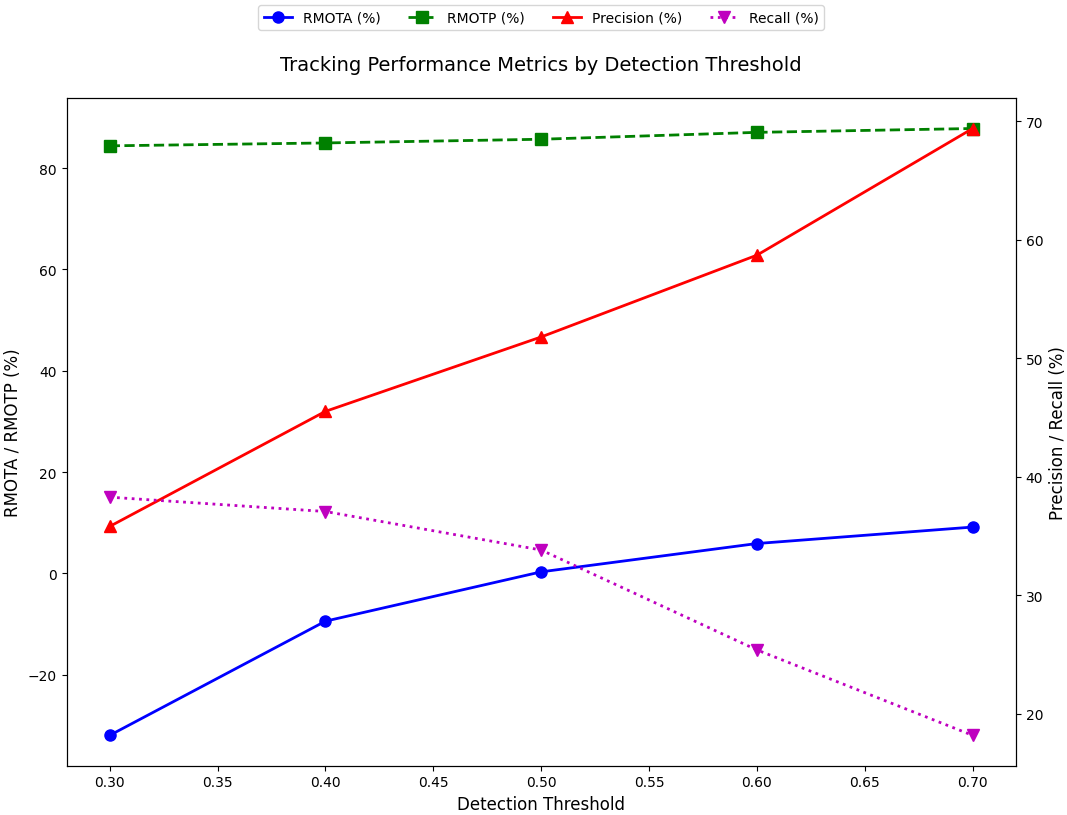
\includegraphics[width=\columnwidth]{picture/picture6.eps}}
	\caption{Analysis of the impact of point cloud detection threshold on multi-object tracking performance. Experiments show that the accuracy and threshold of vehicle detection are the key factors affecting tracking performance.} 
	\label{fig6} 
\end{figure}

\begin{figure}[!t]
	\centering
		\centerline{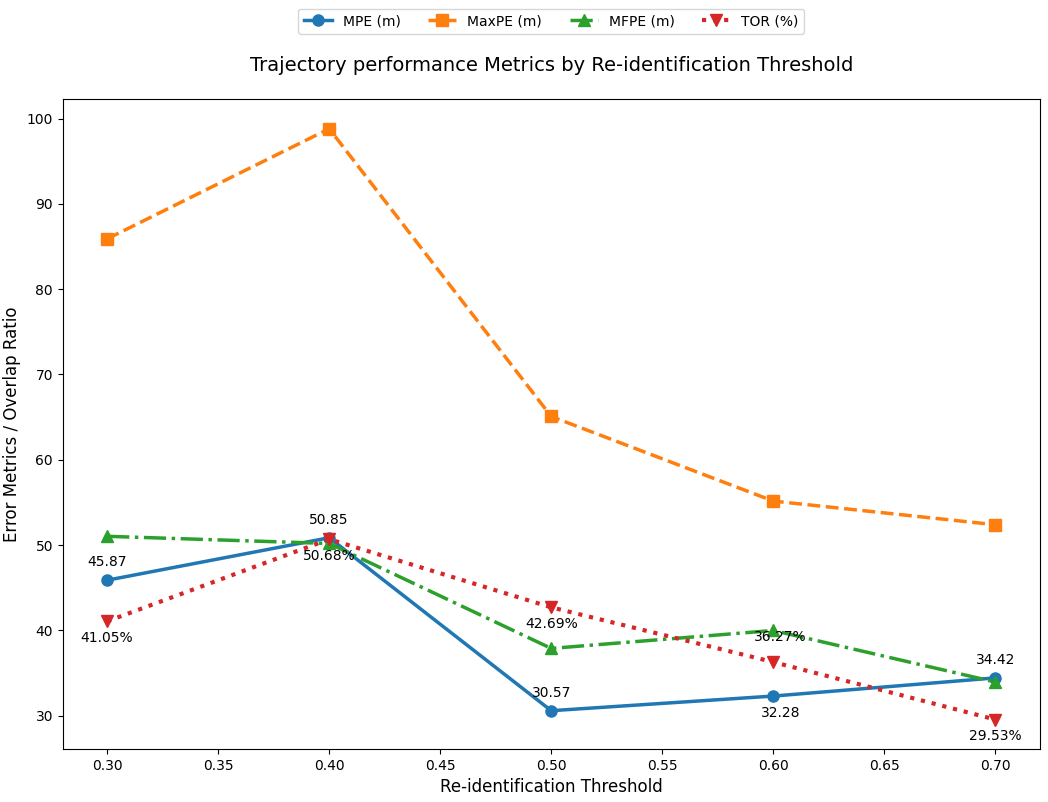
\includegraphics[width=\columnwidth]{picture/picture7.eps}}
	\caption{Comparative analysis of vehicle re-identification threshold effects on trajectory matching accuracy, illustrating the relationship between threshold values and the alignment degree between tracked trajectories and ground truth trajectories in urban traffic scenarios.} 
	\label{fig7} 
\end{figure}

Overall, the tracking performance varies significantly across intersections. Intersection 4 in Town01 achieves high scores for both metrics (\(RMOTA\): 60.2369; \(RMOTP\): 89.0919), while Intersection 5 in Town10 shows notably lower accuracy (\(RMOTA\): 16.7388), indicating weaker tracking reliability.
However, detection accuracy is also affected by the number of vehicles passing through the intersection, and the system accuracy improves significantly in low traffic conditions.
These data highlight the performance variations of the multi-object tracking system across different scenarios and intersections, providing valuable insights for further optimization.

\textbf{Twin.}
The performance of the digital twin is primarily reflected by two sets of metrics: trajectory coincidence and control error (as shown in Table \ref{tab:3}). 
These two tables compare the performance evaluation metrics of the digital twin in two scenarios, Town01 and Town10. 
The TOR in Town01 is significantly higher than that in Town10 in the comparison of the Tracking Trajectory with the Digital Twin trajectory (TT-DT), indicating that it has a superior path tracking ability, which may be due to the simpler environment or the more stable control algorithm.
However, for the comparison between the Tracked Trajectory and Ground Truth (TT-GT), it is higher in Town10, probably because our point cloud dataset was collected in Town10 and is more suitable for vehicle detection in this scenario.
In terms of Mean Position Error (MPE), the two are close (Town01: 79.58m, Town10: 82.41m). 
However, the Maximum Position Error (MaxPE: 105.89m) and Final Position Error (FPE: 105.09m) in Town10 far exceed those in Town01 (MaxPE: 33.14m, FPE: 19.90m), revealing severe localization deviations in extreme cases, likely caused by complex environments or dynamic obstacles. 
For Mean Lateral Error (MLE) and Mean Longitudinal Error (MLOE), Town10 performs slightly better (MLE: 1.98 vs. 2.19, MLOE: 0.26 vs. 0.53), suggesting more precise lateral and longitudinal control, though overall stability is lacking. 
In terms of Mean Delay (MD), Town01 (1.20 seconds) outperforms Town10 (1.38 seconds), demonstrating higher task execution efficiency.

\begin{figure}[!t]
	\centerline{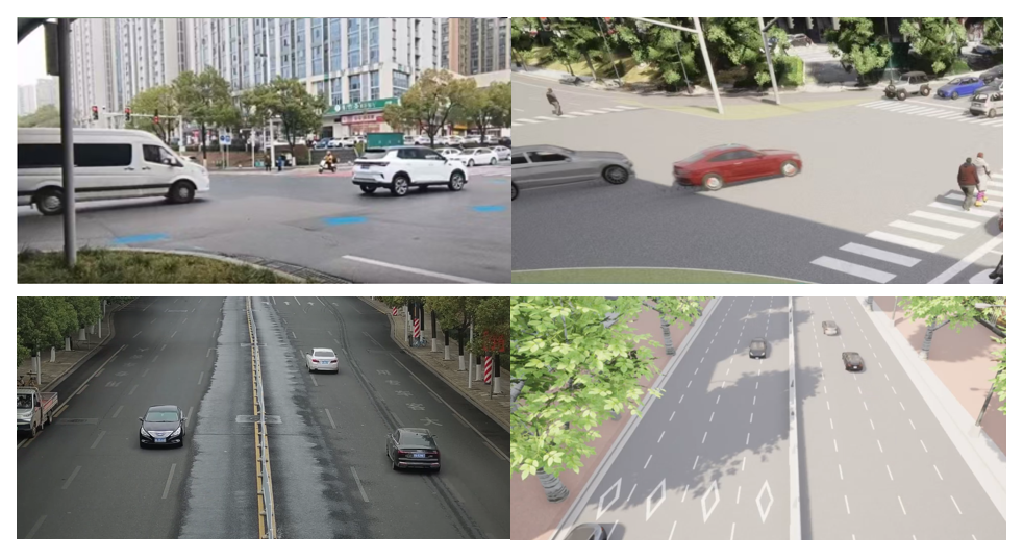
\includegraphics[width=\columnwidth]{picture/picture8.eps}}
	\caption{In addition to the default environments (Town01/Town10) of CARLA, our UVDT framework is successfully deployed in two other custom city scenes. Top: Changsha CEC Software Park. (Left) Real scene; (Right) Digital twin. Bottom: Hunan University of Technology and Business. (Left) Real scene; (Right) Digital twin.} 
	\label{fig8} 
\end{figure}

\begin{table}[t]
	\centering
	\caption{Table of Trajectory Overlap Rate and Vehicle Control Indicators}
	\label{tab:3}
	\renewcommand\arraystretch{1.3}
	\begin{tabular}{|c|c|c|c|c|c|}
		
		\hline
		Scene & Type & TOR(\%) & MPE(m) & MaxPE(m) & FPE(m) \\
		\hline
		\multirow{3}{*}{Town01} & TT-DT & 50.2143 & 79.5798 & 33.1382 & 19.8970 \\
		\cline{2-6}
		& TT-GT & 18.4326 & 59.3773 & 79.6541 & 64.0980 \\
		\cline{2-6}
		& Control & \multicolumn{4}{|c|}{MLE:2.1889, MLOE:0.5345, MD:1.2015} \\
		\hline
		\multirow{3}{*}{Town10} & TT-DT & 10.8957 & 82.4108 & 105.8893 & 105.0854 \\
		\cline{2-6}
		& TT-GT & 34.4533 & 52.5575 & 36.0566 & 31.4600 \\
		\cline{2-6}
		& Control & \multicolumn{4}{|c|}{MLE:1.9835, MLOE:0.2614, MD:1.3780} \\	
		\hline
	\end{tabular}
\end{table}

\subsection{Details Explanation}

We conducted ablation studies on LiDAR detection and multi-intersection multi-object tracking in object detection to ensure that our experiments achieved the desired results.

\textbf{Detecting Vehicles in 3D Point Clouds.}
During the process of detecting vehicles in the 3D point cloud, we set a threshold for the detection results.
Before optimizing the tracker hyperparameters, we conducted multiple experiments in the Town10 scenario, and the experimental results are shown in Fig. \ref{fig6}.
When the threshold is too low, some non-vehicle objects, such as trees and buildings, will be mistaken for vehicles. In some cases, even the cargo loaded on the vehicle will be mistaken for a vehicle, and the recognition accuracy will be greatly reduced.
On the contrary, if the threshold is too high, some vehicles will be missed, such as smaller cars, which are occasionally mistaken for boxes and ignored.
When the threshold is 0.6, there is obvious feature crossover, which is the best choice for comprehensive tracking performance.

\textbf{Multi-Intersection and Multi-Object Tracking.}
In the multi-intersection multi-target tracking experiment, the most critical task is the re-identification of vehicles across different intersections. 
Therefore, we also set a threshold for the re-identification results: if the similarity score exceeds the threshold, the targets are considered the same vehicle; otherwise, they are deemed different vehicles. 
During the experiment, we adjusted the threshold several times in the Town10 scenario, and the experimental results are shown in the Fig. \ref{fig7}.
We use 0.5 as the ReID threshold because it achieves the best balance between security, stability, and scalability, avoiding both the extreme error of a low threshold and the risk of trajectory breakage of a high threshold.

\subsection{Adaptive Data Association Threshold}

\textbf{Background and Objectives.}
In order to further improve the performance of the tracker highly depends with the hyperparameter setting. 
Traditional manual parameter tuning is inefficient and difficult to find the global optimal solution. 
For this reason, we adopt a Bayesian Optimization (BOM) approach to automatically optimize the following key parameters through an intelligent search strategy:

\(\bullet\) DetectionProbability: control the reliability of sensor detection.

\(\bullet\) ClutterDensity: sensitivity to filtering false detections.

\(\bullet\) NewTargetDensity: threshold for target initialization.

\(\bullet\) Confirmation/DeletionThreshold: trajectory lifecycle management.

\(\bullet\) DeathRate: robustness to handling targets leaving the scenario.

Optimization goal: maximize \(RMOTA\) while reducing IDS and trajectory fragmentation.

\textbf{Optimization Processes.}
Bayesian optimization is a hyper-parametric optimization method based on probabilistic models, which solves the global optimization problem of black-box functions by the strategy of “finding the best parameter with the least number of attempts”.
The process is as follows:
1.Maximizing tracking performance by fitting existing data with a Gaussian process and constructing an objective function model in a 6-dimensional parameter space; 
2.A small number of random parameter combinations are selected to calculate the value of the acquisition function, and the next parameter to be tested is selected (e.g., the point with the largest Expected Improvement); 
3.Run the experiment to get the \(MOTA\) corresponding to the new parameters, add to the dataset, and repeat until the maximum number of iterations is reached or convergence is achieved.
The improvement results after optimization compared with before optimization are shown in Fig. \ref{fig4}.   
\begin{figure}[!t]
	\centerline{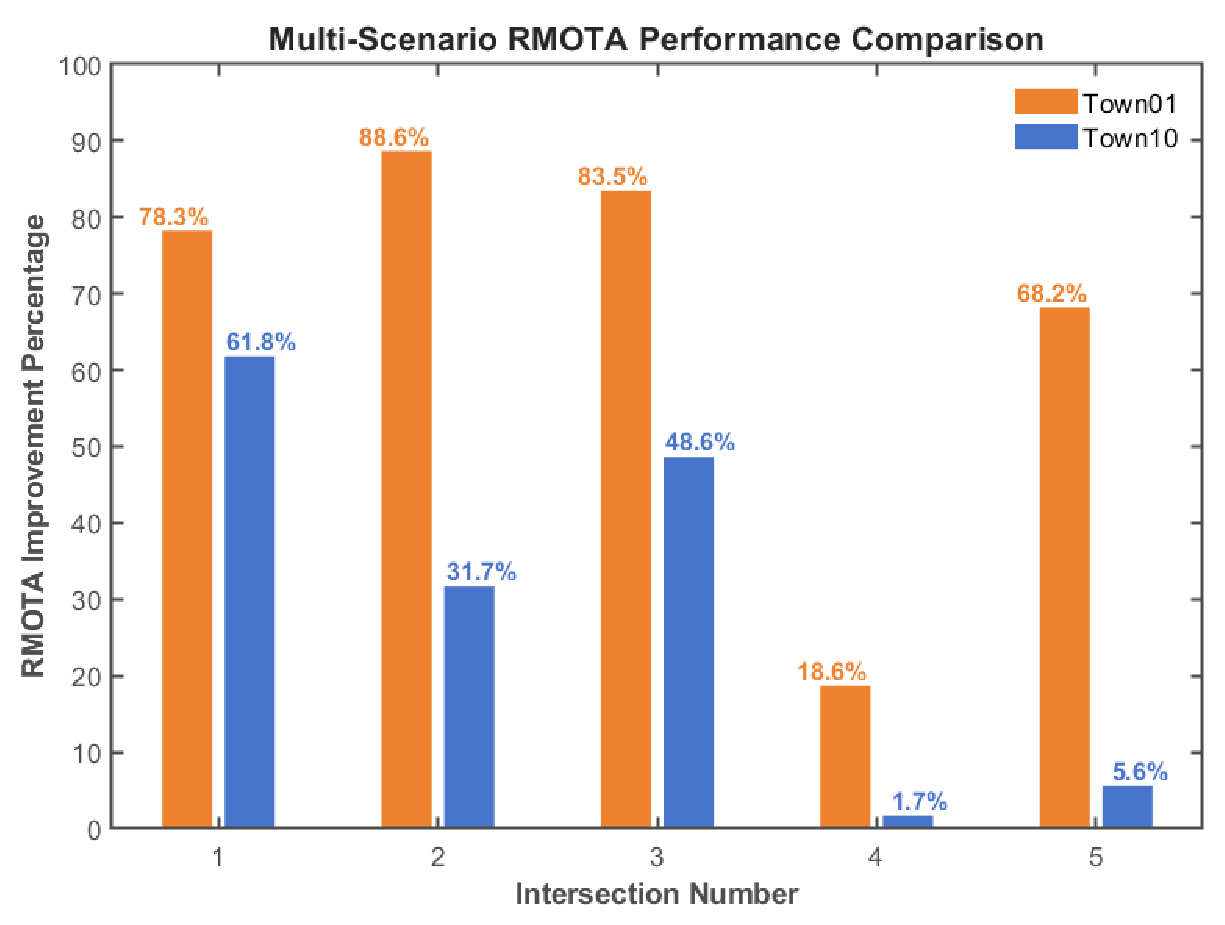
\includegraphics[width=\columnwidth]{picture/picture4.eps}}
	\caption{Comparison of \(RMOTA\) improvement (\%) after hyperparameter optimization on Town01 and Town10. The results demonstrate the effectiveness of the optimization strategies used in different scenarios.} 
	\label{fig4} 
\end{figure}

\subsection{Limitations and Future Directions}

\textbf{Problems Encountered in The Experiment.}
During our experiments, we encountered the following issues:  
1.When matching trajectories across multiple intersections, images of vehicles corresponding to each trajectory are needed to extract re-identification appearance features. 
Acquiring these images is difficult, and the methods used can affect accuracy.  
2.When matching trajectories, it is necessary to associate trajectories from all intersections. 
However, due to ID switching, the trajectory of the same vehicle at a single intersection may be fragmented, making integration complex. 
If only one trajectory is selected as the current intersection's trajectory for a vehicle, issues arise when the same vehicle returns to the intersection.

\textbf{Shortcomings of Current Research.}
As shown in Fig. \ref{fig8}, although our experiments have been replicated in multiple real scenarios, there are still some limitations.
For example, the detection accuracy of PointPillars is not high, resulting in suboptimal tracking performance. 
Additionally, false detections may occur when acquiring images of vehicles corresponding to current trajectories, potentially leading to trajectory matching errors.

\textbf{Vision of The Future.}
Our experiments were conducted under offline conditions, meaning they lacked real-time capabilities. 
If it is to be deployed in practice, it is necessary to overcome engineering challenges such as sensor network scale expansion and parameter adaptive adjustment.
In future work, we aim to transition these experiments to an online framework to achieve high real-time performance, thereby enhancing their experimental value.


\section{Conclusion}

Through a series of experiments, we have demonstrated the application value of UVDT in intelligent transportation. 
Digital twin technology can not only accurately replicate real-world traffic scenarios but also effectively predict future traffic conditions. 
Multi-object tracking and the inference of unknown trajectories serve as strong evidence of this capability. 
This holds significant value for the development of future cities.
We hope that new large-scale datasets will be introduced in the future to further enhance the effectiveness of digital twins.

\section{Acknowledgements}
The authors gratefully acknowledge the financial support provided by the Natural Science Foundation of Hunan Province (No.2024JJ6190), Research on a new generation of brain-like intelligent computing framework based on ultra-large-scale real neural systems (No.24XJJCYJ01001), Scientific research project of Hunan Provincial Department of Education (No.22B0646), the Open Project of Xiangjiang Laboratory (No.23XJ03009), Xiangjiang Laboratory key project subproject (No.22XJ01001-2), the “Digital Intelligence +” interdisciplinary research project of Hunan University Of Technology and Business (No.2023SZJ19).

\bibliographystyle{IEEEtran}
\bibliography{reference}


\begin{IEEEbiography}[{
\includegraphics[width=1in,height=1.25in,clip,keepaspectratio]{authors/HaidongWang/HaidongWang.eps}}]{Haidong Wang} received the B.E. degree in Computer Science and Technology from Hunan University Of Technology and Business, Changsha, China, in 2014, the M.Sc. degree in Computer Technology from the University of Chinese Academy of Sciences (UCAS), Beijing, 	China, in 2017, and Ph.D. degree in Hunan University, Changsha, China. His current research interests include brain-like vision, deep learning and reinforcement learning.
\end{IEEEbiography}

\begin{IEEEbiography}[{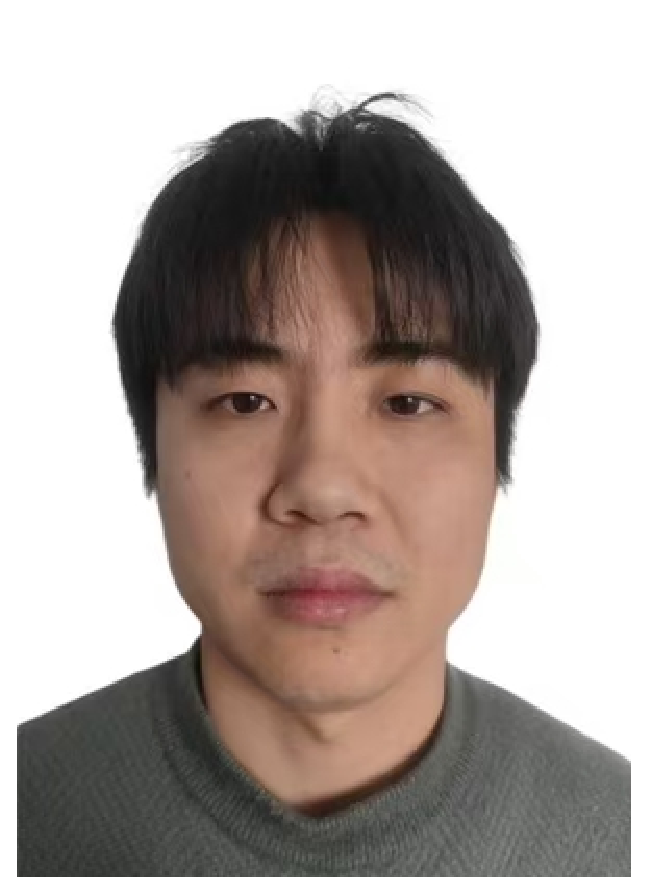
\includegraphics[width=1in,height=1.25in,clip,keepaspectratio]{authors/PengfeiXiao/PengfeiXiao.eps}}]{Pengfei Xiao} received the B.E. degree in Computer Science and Technology from Changsha College, China, in 2022, and is now studying in Hunan University of Commerce and Industry, Changsha, China, pursuing a professional type master's degree in Computer Technology. His current research interests include brain-like perception, deep learning and autonomous driving.
\end{IEEEbiography}

\begin{IEEEbiography}[{
\includegraphics[width=1in,height=1.25in,clip,keepaspectratio]{authors/AoLiu/AoLiu.eps}}]{Ao Liu} received the B.E. degree in Computer Science and Technology from Changsha College, China, in 2023, and is now studying in Hunan University of Commerce and Industry, Changsha, China, pursuing a professional type master's degree in Computer Technology. His current research interests include brain-like control and deep learning.
\end{IEEEbiography}

\vfill\null
\newpage
\begin{minipage}[t][0pt][t]{0.48\textwidth}
	\vspace{-10ex}
	\begin{IEEEbiography}[{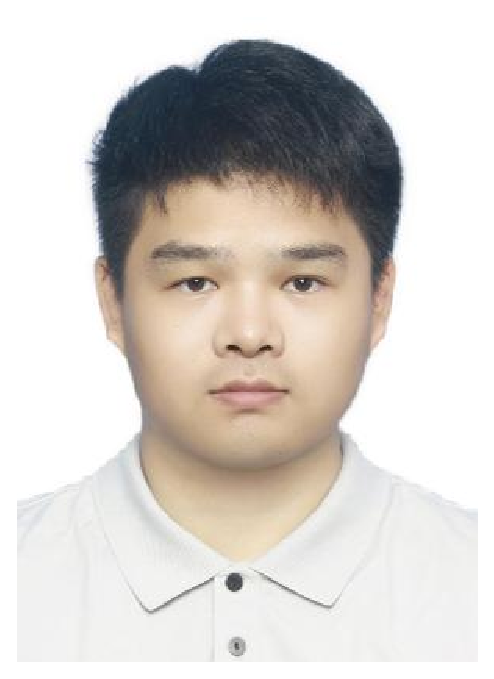
\includegraphics[width=1in,height=1.25in,clip,keepaspectratio]{authors/QiaShan/QiaShan.eps}}]{Qia Shan} received the B.E. degree in Network Engineering from Hainan University, Haikou, China, in 2020, and is currently pursuing the M.Sc. degree in Software Engineering at Hunan University Of Technology and Business, Changsha, China. His current research interests include brain-like affective computing and deep learning.
	\end{IEEEbiography}
	
	\begin{IEEEbiography}[{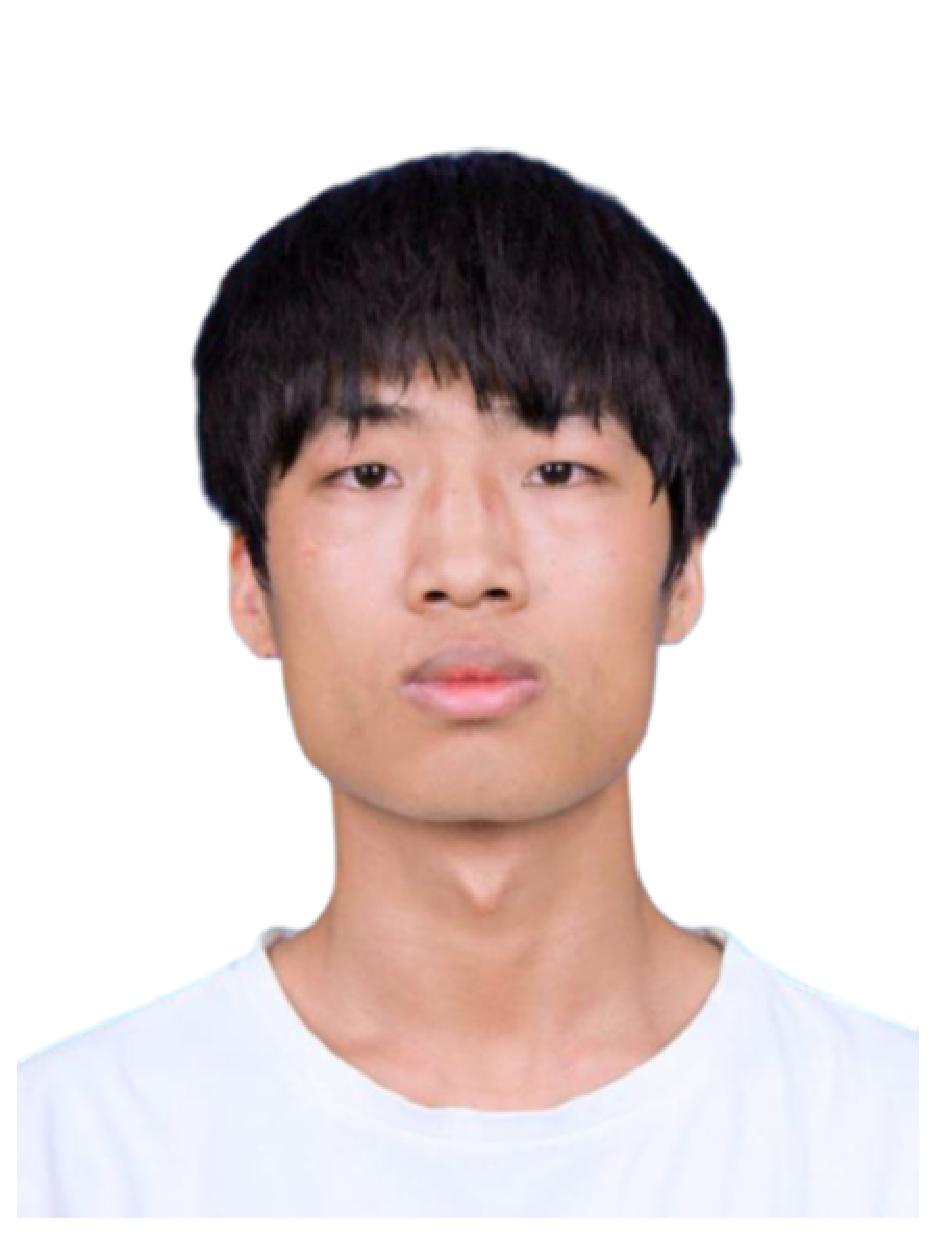
\includegraphics[width=1in,height=1.25in,clip,keepaspectratio]{authors/JianhuaZhang/JianhuaZhang.eps}}]{Jianhua Zhang} received the B.E. degree in Software Engineering from Taiyuan University of Technology, TaiYuan, China, in 2022,and M.Sc. degree in Software Engineering from the Hunan University Of Technology and Business, Changsha, China. His current research interests include brain-like vision and deep learning.
	\end{IEEEbiography}
    \vspace{\fill} % 弹性填充剩余空间
\end{minipage}
\end{document}
